\chapter{Background and Related Works to the Embracing Sphere}
    This chapter establishes fundamental concepts related with Embracing Sphere by covering in-depth environmental storytelling, acoustics and haptics. The chapter aims to investigate artworks and video games chosen for their relation to the Embracing Sphere on both conceptual and practical levels.\par
    \section{Environmental Storytelling and Developments in Virtual Environments}
        Discussions about environmental storytelling as a term in narratology dates back not so long ago. First defined in 2000 by Don Carson, a former theme park designer for Walt Disney Imagineering, argues that in themed environments “the story element is infused into the physical space a guest walks or rides through”\cite{Liminal_Space_Between_Embedded_and_Emergent_Narrative}. During his work in theme park train rides or video games, his objective to tell a story through the experience of traveling through a real or imagined physical space\cite{Lessons_Learned_from_the_Theme_Park_Industry}.\par

        These discussions later developed into a game design discourse as concept of "story versus play", "ludology vs narratology\cite{Hamlet_on_the_Holodeck}" within transmedia storytelling\cite{Jenkins_Shall_We_Play}. Jenkins argues that the story becomes richer and more complex, as the audience is given more opportunities to engage with the narrative.\par

        Although the transmedia storytelling directs something else (a process where integral elements of a fiction get dispersed systematically across multiple delivery channels\cite{Jenkins_Transmedia}) a discussion of the narrative potential of video games supported attempts to create narrative spaces in virtual environments\cite{Liminal_Space_Between_Embedded_and_Emergent_Narrative}.\par

        \subsubsection{Case Study: Journey}
            \emph{“Like a religious ritual of passage, it is not the spiritual narrative’s plot, but rather the poignant symmetry between its metaphorical meaning. The embodied experience of performing the movements it channels, that makes this narrative effective. Journey makes zero use of language and relies entirely on the experience of movement to tell its story\cite{Game_Movement_as_Enactive_Focalization}\cite{Narrative_Geography}.”}\par

            \begin{figure}[H]
                \centering
                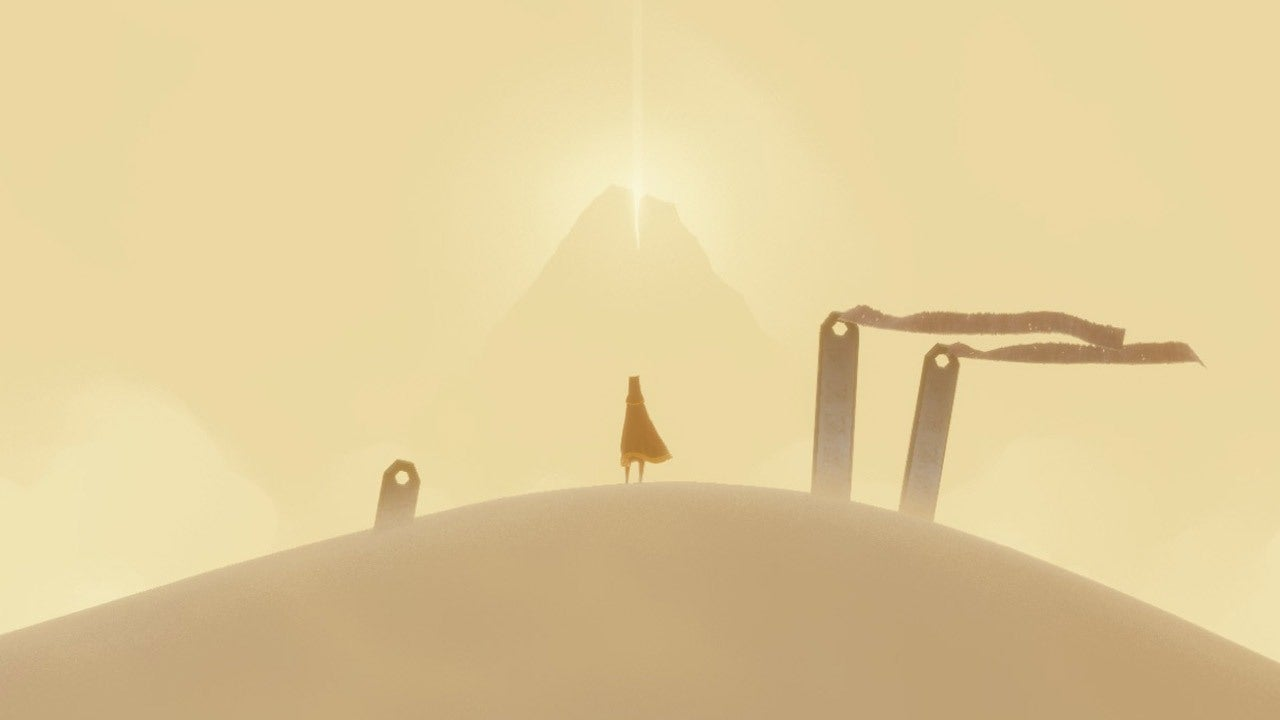
\includegraphics[width=0.8\textwidth]{images/journey.jpg}
                \caption{A visual from the game called Journey released in 2012 by Thatgamecompany and Santa Monica Studio.}
                \label{fig:JOURNEY}
            \end{figure}

            Environmental storytelling in video games done by staging the game world so that the arrangement of objects, scenery and audio cues naturally conveys story to the player\cite{BioShock_Infinite}.\par

            Journey is a video game has critic focus on exploration and a great, well awarded (Journey won several "Game of the Year" awards from different organizations) example for environmental storytelling. The game accomplishes this narrative success mostly by not relying any use of linguistics or semantics.\par

            In Journey, the player controls a figure starting in a vast desert, traveling towards a mountain in the distance in a multiplayer environment, which means you as a player can meet interact with other players on the same journey. The challenge is, players cannot communicate via speech or text and cannot see each other's names until after the game's credits.\par

            Players have basic navigational controls like walking, jumping, sliding on the dunes and ability to emit a wordless shout to another. The length and volume of the shout depends on how the button is pressed.\footnote{Journey shout example: \url{https://youtube.com/clip/UgkxMXBXc4aZmHuOL2f3PUoEVQ57Og5Suyks/}}\par

            Through the players path in Journey, one distinct element always catches eye. The big shining mountain peak in the horizon, pictures an unspoken, ultimate goal or a direction for our journey. Each player trying to reach the peak either by helping each other or going this path individually.\par

            \begin{figure}[H]
                \centering
                \includegraphics[width=0.8\textwidth]{images/journey_mountain.png}
                \caption{The mountain in the video game, Journey.}
                \label{fig:JOURNEY_MOUNTAIN}
            \end{figure}

            The subtractive design of Journey's game environment forcing player to focus on the environment all the time. Directing to consume story through cryptic glyphs, symbols and figures carved into the walls, artistically placed in the game environment.\par

            By collecting these symbols, players gain more movement ability to explore deeper in the game. This mechanic also shown in diegetic way with a scarf wrapped around the player characters head. The scarf is giving information about your energy left to jump and fly around like the fuel in your tank or stamina left. The scarf grows as you progress through the game by picking up collectible symbols.\par

            \begin{figure}[H]
                \centering
                \includegraphics[width=0.8\textwidth]{images/journey_scarf.png}
                \caption{The player's scarf in the Journey.}
                \label{fig:JOURNEY_SCARF}
            \end{figure}      

            In Journey, the narrative aspect of the non-linguistic communication and the movement through the designed space, generates the story. The player reconstructs the story by interpreting different objects in ruins, interacting with the others and initializing events embedded in the game environment.\par

            Video game in that sense has one characteristic feature, which is their spatiotemporality. In comparison to other multimedia mediums like cinema which is purely temporal sequences, we can view video games narrative as a blend of the temporal and the spatial\cite{Liminal_Space_Between_Embedded_and_Emergent_Narrative}.
        \subsection{Existing Environmental Storytelling Methods in Different Mediums}
            Environmental storytelling is not entirely specific to video games. First in theaters then later adopted in screenplay, there is a French term called "mise-en-scene" in literal translation "putting into the scene". Mise-en-scene describes the arrangement of scenery, props, lighting and other visual elements to support the story. Filmmakers and production designers use settings to provide backstory and mood. For example, a character’s cluttered apartment, lit by a flickering lamp, can imply their personality and situation before they even speak. In cinematic terms, every object in the frame is there by choice to serve the narrative.\cite{Mise_en_scene}\par
        
            Details like wall posters, broken objects or photographs can signal past events. A close-up of a train ticket on a nightstand might hint where a character planned to go. In film theory, such embedded clues function like visual foreshadowing. Viewers can pick up these details either consciously or subconsciously. Production designers and directors use every element of mise-en-scene to make the environment feel lived-in and story-rich.\par
            
            For the comparison between cinema and video games, we can broadly categorize video game narrative broadly into 2 categories: "embedded narrative", which follows pre-authored contents as temporal narrative sequences that still exist without audience action and "emergent narrative" which is directly linked with audiences meaningful action, exploration and interaction with the virtual environment\cite{Liminal_Space_Between_Embedded_and_Emergent_Narrative}. Cinema, doesn't have emergent narrative due to its fixed media characteristics. According to Natalia A. Bracikowska, environmental storytelling exist in liminal space between embedded and emergent narrative\cite{Liminal_Space_Between_Embedded_and_Emergent_Narrative} and this aspect of environmental storytelling opens a pretty viable path to convey multi-branched story bits for the audience.\par
            
            Across interactive media, game design and film theory, environmental storytelling is a shared strategy to embed narrative in the space itself. In all domains, meaning is conveyed indirectly. Games and interactive media emphasize the user’s role in uncovering that meaning players must explore and investigate to “do the work” of interpretation. In contrast, films present a fully authored scene but still rely on designed space to impart story context. There is a common goal to see, which is to make every detail of the world serve the story.\par
        \subsection{Auditory Environmental Storytelling}
            \emph{"Sound is a integral part of every performative and aesthetic experience with an artifact. Yet, in design disciplines, sound has been a neglected medium, with designers rarely aware of the extent to which sound can change the overall user experience."\cite{Sonic_Interaction_Design}}

            According to Stefania Serafin, humans are sensitive to sounds arriving from anywhere within the environment whereas the visual field is limited to the frontal hemisphere, with good resolution limited specifically to the foveal region. Therefore, while the spatial resolution of the auditory modality is cruder, it can serve as a cue to events occurring outside the visual field-of-view\cite{Sonic_Interaction_in_Virtual_Environments}. Therefore effective auditory environmental storytelling relies on a sophisticated understanding of how different sound elements function individually and collectively to shape the user experience.\par

            The concept of "presence" and "immersion" highly relates with this subject in perspective of auditory domains characteristics on fully spherical perception and cognition.\par

            Immersion is a studied in multiple different field such as film, video games and music. It is a subject that can have different meaning depending on the context of the field of study\cite{Sonic_Interaction_in_Virtual_Environments}. Immersion is a metaphorical term that derived from the physical experience of being surrounded. In Janet H. Murrays words, "being submerged in water"\cite{Hamlet_on_the_Holodeck}. 

            Presence on the other hand is a term that used in much broader sense. According to Lombard and Ditton, presence described as the feeling of “being there” in a mediated environment, even though the experience is happening through a screen or device. Presence can occur in different forms, such as feeling physically in a place shown on screen, socially connected to others through media, or involved in an environment that reacts to one’s actions\cite{Concept_of_Presence}.

            By understanting how we naturally interact with the world, how we interpret information provided by sensory stimulations, we can apply this understanding to enhance and elevate the immersion and presence in our intended mediums.\par

            Therefore auditory stimulation by its nature, envelopes a lot of human sensory aspects. It is explicitly useful for its spatiotemporal narrative capabilities. With a case study that explores a video game called Return of the Obra Dinn we can have deeper understanding on auditory environmental storytelling.\par
        \subsubsection{Case Study: Return of the Obra Dinn}
            Return of the Obra Dinn, is a adventure-puzzle video game developed by Lucas Pope in 2018. In the backstory of the game, The Obra Dinn, a merchant ship missing for five years, has reappeared off the coast of England with no known surviving crew or passengers. Players task is to determine every crew members fate, including their names, how they met their fate, who or what killed them and if anybody alive, where are they?\par

            \begin{figure}[H]
                \centering
                \includegraphics[width=0.8\textwidth]{images/ship_02.png}
                \caption{A visual of the ship deck from the game called, Return of the Obra Dinn released in 2018 by Lucas Pope.}
                \label{fig:SHIP}
            \end{figure}

            Players can hop onto the Obra Dinn and navigate on the main deck. The main mechanic portrayed with a latin phrase, "Memento Mortem", a mystical pocket watch that allows the investigator to witness the final moments of any corpse discovered aboard the ship.\par 

            \begin{figure}[H]
                \centering
                \includegraphics[width=0.3\textwidth]{images/pocketwatch.png}
                \caption{A visual of the pocketwatch in Return of the Obra Dinn.}
                \label{fig:POCKETWATCH}
            \end{figure}

            When player approach to a remaining of a crew member the pocket watch can be activated and it triggers a sequence that includes 2 parts: first, an audio snippet right before the event happened, secondly a static, frozen explorable visual tableau of the event that results the death scene.\par

            \begin{figure}[H]
                \centering
                \includegraphics[width=0.8\textwidth]{images/ship.png}
                \caption{A visual of the of a remaining of crewmember in Return of the Obra Dinn.}
                \label{fig:CREWMEMBER}
            \end{figure}

            The crew member shown in the \ref{fig:CREWMEMBER} is our first case to solve in this adventure-puzzle game. As we interact with the body remain, a musical cue transport us to the past and we hear an audio snippet\footnote{Return of the Obra Dinn, first audio snippet: \url{https://youtu.be/UXC6Sjsedcg}} which transcription is like that:\par
            \emph{
                \newline
                - "Captain! Open the door..."\newline
                - "Kick it in!"\newline
                - "...lest we break it down... ...and take more than those shells."\newline
                - "You bastards may take... ...exactly what I give you.[DOOR OPENING AND GUN SHOT]"\newline
                }

            \begin{figure}[H]
                \centering
                \includegraphics[width=0.8\textwidth]{images/static_scene.png}
                \caption{A visual the static scene of Return of the Obra Dinn.}
                \label{fig:STATICSCENE}
            \end{figure}            

            At the point \ref{fig:STATICSCENE} we have enough sensory cues to solve at least 1 crew members identity which is the Captain himself and we have enough hints to define how this crew member died. Because according to the auditory cues one crew member calls "Captain!" and knocking the door in anger. The other crew member is suggesting to kicking the door and forcefully get into the room. The only person we hear behind door opens it and shoots one of the rebellious crew member immediately.\par

            \begin{figure}[H]
                \centering
                \includegraphics[width=0.8\textwidth]{images/crewmembers.png}
                \caption{An illustration of all crew members of the Obra Dinn.}
                \label{fig:SHIPCREW}
            \end{figure}   

            While the visual scene is frozen, the audio snippet captures the ambient soundscape of that specific moment and location. This ambient layer logically contributes to differentiating scenes and grounding the abstracted visual tableaus in a more tangible sense of place. It is in my perspective, a well done auditory environmental storytelling.\par           

            My experience with this video game was a great inspiration for Embracing Sphere after all. It showed me the possibility of environmental storytelling is indeed strong and it has benefits for spatiotemporal story cases.\par

            After covering necessary perspective from narratology and video game studies, sound and perception are going to be investigated in more detail, specifically acoustics and psychoacoustics subjects within the next subchapter.
    \section{Space and Acoustics in Artistic/Scientific Perspective}
            \emph{"Sound is something most people take for granted. Our environment is full of noises, which we have been exposed to from before birth. What is sound, how does it propagate and how can it be quantified?"\cite{Acoustics_and_Psychophysics}}\par 

            The purpose of this subchapter is to introduce fundamental knowledge ground for room acoustics and describe the usage of room impulse responses in the Embracing Sphere context.\par
        \subsection{Definitions for Room Acoustics}
            Sound is simply a mechanical disturbance of the medium. Medium in that context may be air, solid, liquid or other gas matters. Dependent on the mediums state, the sound can be propagated and while this propagation happens it interacts with physical objects and other sound waves. In room acoustics the interactions of the sound with the medium, basically can be listed as refraction, absorption, reflection and interference. Psychoacoustics is the study how humans perceive sound after all these interactions with the medium\cite{Acoustics_and_Psychophysics}.\par

            The heard sound, is the result of all these complex physical interactions in the place our ears are located.\par

            When sound moves through a room, its behavior is shaped by how it interacts with surfaces, mainly through absorption and reflection. Sound reflection occurs when sound waves hit a hard boundary and bounce back into space. In contrast, sound absorption is when a material takes in the sound's energy, which is converted into small amounts of heat through internal friction, reducing the amount of sound that reflects\cite{Acoustics_and_Psychophysics}. For example, a wooden surface absorbs more sound than a rough concrete one. These interactions, along with others like refraction and interference, collectively determine the acoustic character of a room.\par

            These interactions do not occur in isolation. They collectively define the complex behavior of sound waves and their propagation within the room. Each time a sound interacts with a surface in a room it loses some of its energy due to absorption and reflection. The time that it takes for a sound to gradually fade out in a room is called the reverberation time.\par

            Reverberation time is an important aspect of sound behavior in a room. Mentioned different absorption coefficient values in different materials and frequencies shapes the perception of the room. If the sound dies away very quickly, we perceive the room as being “dead” or if the sound dies away very slowly, we perceive the room as being “live”. To calculate reverberation times there is a simple formula known as the “Sabine formula”, named after its developer Wallace Clement Sabine\cite{Acoustics_and_Psychophysics}.\par 
            $$RT_{60} = \frac{0.161 \cdot V}{A}$$
            \begin{itemize}
                \item RT60: This is the reverberation time in seconds. It's defined as the time it takes for the sound pressure level in a room to decrease by 60 decibels (dB) after the sound source has stopped\cite{Room_Acoustics}.
                \item 0.161: This is a constant. Its units are seconds per meter (s/m). This constant is derived empirically and is based on the speed of sound in air at a typical room temperature.
                \item V: This represents the volume of the room in cubic meters. Calculated by multiplying the length, width and height of the room.
                \item A: This is the total sound absorption of the room in Sabins. It's calculated by summing the absorption of all surfaces in the room. The absorption of each surface is found by multiplying its surface area in square meters by its sound absorption coefficient at a specific frequency.
            \end{itemize}

            According to the Sabine formula, reverberation time depends on the volume, surface area and the average absorption coefficient in the room. However, the absorption coefficients of real materials are not constant with frequency. This difference in absorption strength in different frequencies changes heard timbre of the room as the sound in the room decays away. Apart from being useful, Sabine formula has assumptions for speed of sound and static response of the reflective materials in the room. To more accurately measure reverberation time, another method called room impulse response capturing was introduced in 1964 by M. R. Schroeder \cite{New_Method_Measuring_RT}.\par

            This method uses tone bursts (or filtered pistol shots) to excite the enclosure (room). The captured smooth decay curves resulting from the new method improve the accuracy of reverberation time measurements and facilitate the detection of non-exponential decays\cite{New_Method_Measuring_RT}.\par

            These impulse response recordings can be used later to reconstruct a virtual environment with the same reverberation curves as captured room with a mathematical operation called convolution. An anechoic (no reflections) sound is convolved with an RIR and this mathematical process applies the room's acoustic snapshot to the sound. The convolution effectively embeds the reflections and reverberation captured in the RIR to the original sound.\par
        \subsection{Room Impulse Response Measurement Methods}
            \emph{"Between stimulus and response there is a space. In that space is our power to choose our response. In our response lies our growth and our freedom."\cite{Sonic_Interaction_in_Virtual_Environments}}

            The quote above is highly controversial because it has been referred to an Austrian neurologist and psychologist, Viktor Frankl by Stephen R. Covey in his book called The Seven Habits of Highly Effective People but quote that referred to Frankl's book, Man’s Search for Meaning hasn't got any line that includes the quote. Although I wanted to share this quote as a poetic mood setter for this chapter.\par

            From an artistic perspective, Embracing Sphere refers to this metaphorical concept of relation between stimulus and response of space. Either directly or metaphorically it is powerful representation in spatial perception. Embracing Sphere is about creating an environments/spaces that are capable of telling stories. These spaces should contain both stimulus and response. Although in Embracing Sphere, audience doesn't have power of choice, space has that power because I view the space as an actor that has a lot to tell. The response of the space, grows and establish its freedom.\par

            Acoustics, mathematics, methodologies around it can be covered so deep in details but in the end all of these descriptions and formulas exist in my research to support my artwork to understand the background and design choices of the Embracing Sphere. Therefore RIRs are important in my artwork to give acoustic and spatial context to the audience. It is useful to render the depth and the aural character of the environment into audio content.\par

            In previous sections we covered room impulse response description in surface level. It is a captured audio file that contains acoustics space characteristics such as frequency changes, reverberation decay and length.\par

            There are several practical ways to capture RIR of a room. The easiest one is popping a balloon in the desired room and recording the balloon pop. This method is practical but not much accurate and it is not easy to re-create again because every balloon pop sound parameters can be differ in frequency-wise\cite{RIR_Swept-Sine_Technique}. The more accurate method is sine sweep technique\footnote{A sine sweep IR capture example: \url{https://youtu.be/1egKAtC16e8?feature=shared}}, which includes 1 reference sine wave sweep audio (5-10 seconds long) that starts from 20Hz and sweeps every frequencies until 20kHz\cite{Auditory_Perception_of_Sound_Sources}. In this method the room is acoustically excited by this sine wave and with a microphone the room response recorded then processed with a mathematical process called deconvolution that extracts RIR with subtracting reference sine sweep from reverberant recording.\par

            \begin{figure}[H]
                \centering
                \includegraphics[width=0.8\textwidth]{images/IR_Capture_Balloon_Pop.png}
                \caption{A visual from a recording session for capturing room impulse response in an old house in Balat, Istanbul.}
                \label{fig:IR_BALLOON}
            \end{figure}            

            The visual in \ref{fig:IR_BALLOON} is a recording session in 2021 when I was working as an audio designer in a company called Vadi Sound. In that frame we were capturing RIR with balloon popping in an old house in Balat, Istanbul. The house specifically interesting for capturing RIR because it was one of the few historical wooden houses remain in the Istanbul from early Turkish Republic times. In that situation we hadn't got any high quality full range speaker to excite the room so we choose to pop a balloon at several places in the room to capture as many different positions RIR.\par

            \begin{figure}[H]
                \centering
                \includegraphics[width=1\textwidth]{images/IR_Capture_Sine_Sweep.png}
                \caption{A visual of a RIR capturing session in a studio using sine sweep method. Retrieved from Audioease website \url{https://www.audioease.com/altiverb/browse.php}}
                \label{fig:IR_SINE}
            \end{figure}

            An RIR capturing session that using sine sweep method can be seen in the figure \ref{fig:IR_SINE}. The specific setup uses 2 omnidirectional microphone positioned in the A/B stereo miking technique (a well known stereo miking technique in ambience recordings.)\cite{Sound_Reinforcement}\cite{Professional_Microphone_Techniques} and 1 binaural microphone to capture studio room impulse response.\par

            \begin{figure}[H]
                \centering
                \includegraphics[width=0.4\textwidth]{images/Room_RT.png}
                \caption{An illustration of raytracing of a sound in a close environment. Drawn in AMROC website \url{https://amcoustics.com/tools/amray}}
                \label{fig:IR_RAYTRACE}
            \end{figure}

            Either method works in basic principle shown in the figure \ref{fig:IR_RAYTRACE}. A source that exciting the room and a capturing point that captures the room's acoustic character.\par

            RIRs are artistically useful for virtual aural architecture. In real life architecture uses volumes to evoke intended emotion or paradigms. Some spaces can evoke feeling about privacy or loneliness, others can invite for social cohesion or some space can establish an hierarchy between different roles in the society\cite{Spaces_Speak_Are_You_Listening?}. Artistically I see enclosed spaces and its response as an actor in my story. Same dialog or sonic events can convey many different meanings and feelings according to environments relation with the stimulation.\par

            \begin{figure}[H]
                \centering
                \includegraphics[width=1\textwidth]{images/IR_Comparison.png}
                \caption{Plotting of RIR files of 2 distinct spaces, a small room and The Hagia Sophia. Plotted with matplotlib and librosa in python.}
                \label{fig:IR_COMP}
            \end{figure}

            To explain frequency difference and reverberation time affect in any sonic event, the 2 completely different character RIR waveform and spectrogram graphic shown in the figure \ref{fig:IR_COMP}. As we can see at the left column in the graph, these 2 RIR files has quite different in length and density.\par

            First row with blue waveform is from a small room RIR shown above with a picture of mine holding a balloon. The length of this small room RIR is around 500ms which indicates small volume and highly absorbent environment with carpets on the floor, many cushions and curtains.\par 
            
            The second row with orange waveform is from architecturally and historically famous building Hagia Sofia in Istanbul built in 6th century. The Byzantine church Hagia Sophia transformed into a mosque after conquest of Constantinople (modern day Istanbul) by Ottoman Empire in 1453 and functioned as a mosque until it transformed into a secular museum with the political and social reforms made in 1935 under Mustafa Kemal Atatürk then reverted back into a mosque in 2020 by Turkish government to support their religious ideologies and symbolic political endeavors\cite{Evolution_of_Hagia_Sophia}. This iconic wonder has stood against time and many diverse cultural influences.\par

            To study the acoustics of old Byzantine churches and mosques built by famous architect Sinan (known as Mimar Sinan) the CAHRISMA project (Conservation of the Acoustical Heritage by the Revival and Identification of the Sinan’s Mosques Acoustics) started in 2003\cite{Hagia_Sophia_Multisensory_Aestethics}. In this project, sine sweep technique used, a omnidirectional loudspeaker emits a sinusoidal sweep signal in the Hagia Sophia and the response of the environment is simultaneously recorded with a microphone. The sweep response is then deconvolved with the reference sweep signal\cite{Odeon_Hagia_Sophia}.\par

            \begin{figure}[H]
                \centering
                \includegraphics[width=0.6\textwidth]{images/hagia_sophia_wireframe.png}
                \caption{Wireframe visualization of Hagia Sophia from ODEON software. Retrieved from ODEON web-blog \url{https://odeon.dk/the-church-hagia-sophia}}
                \label{fig:HS_WIREFRAME}
            \end{figure} 

            The RIR of Hagia Sophia then the analyzed and full acoustic model built in an acoustic software called ODEON\cite{Odeon_Hagia_Sophia}. This model can simulate auralization of any anechoic sound inside Hagia Sophia in different positions and the aural difference between Hagia Sophia as a mosque (with carpet floor and wooden panels with Arabic inscription) and Hagia Sophia as a church (mainly marble floor, stone walls)\cite{Revived_Acoustical_History_of_Hagia_Sophia}.\par

            \begin{table}[h!]
                \centering
                \begin{tabular}{|l|c|c|c|c|c|}
                \hline
                Material & 125 Hz & 250 Hz & 500 Hz & 1000 Hz & 2000 Hz \\
                \hline
                Painted Wood & 0.04 & 0.04 & 0.07 & 0.06 & 0.06 \\
                Carpet       & 0.01 & 0.02 & 0.06 & 0.15 & 0.25 \\
                Marble       & 0.01 & 0.01 & 0.01 & 0.01 & 0.02 \\
                \hline
                \end{tabular}
                \caption{Absorption coefficients for painted wood and marble at different frequencies\cite{Absoption_Coefficient_Table}.}
                \label{tab:COEFF}
            \end{table}

            As we see the shown in the figure \ref{fig:IR_COMP} Hagia Sophia's reverberation time is much longer than than our small room, around 6-8 seconds. The frequency response of both of the examples also shown in the figure \ref{fig:IR_COMP}. The frequency response also depends on volume, absorption coefficient and affects the heard sound dramatically. High frequencies are easier to absorbed by air and surfaces\cite{Room_Acoustics} in the room and this can be seen in the figure \ref{fig:IR_COMP} as a colorful slope in the spectrogram panels in the right column.\par

            In artistic view, ability to snapshot an environment and using for creating virtual environments\cite{Recreation_of_the_Acoustics_of_Hagia_Sophia} highly interesting and useful for my perspective. Using RIRs to develop such virtual environments require a specific signal processing called "convolution". The next section will cover the practical mathematical description of convolution and its capabilities in digital audio.            
        \subsection{Convolution in Math and Digital Audio}
            Convolution is a mathematical operation that combines two functions to produce a third function. This new function expresses how the shape of one function is modified by the other. In simple terms, convolution tells us how one signal changes when it passes through a system described by another signal. The convolution algorithm is often interpreted as a filter, where the kernel filters the feature map for certain information\cite{Deep_Learning_Core_Concepts}.\par

            We can say that convolution is fancy multiplication\cite{Guide_to_Convolution}. It is important in physics and mathematics as it defines a bridge between the spatial and time domains and the frequency domain through the convolution theorem. Convolution is essentially used in computer graphics, digital signal processing and lately in machine learning algorithms.\par
            $$(f \ast g)(t)=\int_{-\infty}^{\infty} f(\tau) g(t-\tau) d \tau$$
            The above formula is the formal definition of convolution operation. Instead of starting a calculus lecture, we can present a metaphoric example to deepen our understanding:\par

            Let's say you are running a restaurant. In this restaurant you have a fixed menu and your kitchen uses 2 eggs for one meal. In monday rush hour, 10 meals are ordered in the first hour, 11 in the second, and 12 in the third. How many eggs did you used? It's simple multiplication. 
            $$(2\cdot10)+(2\cdot11)+(2\cdot12)=66$$
            The answer is 66 but in Tuesday your chef added a dessert that requires an egg to make. Desserts are getting served after 1 hour of each meal. How many eggs you use for each hour? This is now a complex problem because the eggs amount overlaps after first hour.

            First hour is simple you prepare initially 10 meals with 2 eggs each. 
            $$2\cdot10=20$$
            Then the next hour you have to prepare 11 meal but also 10 desert for the visitors from first hour.
            $$(2\cdot11)+(1\cdot10)=32$$
            The third hour after your last visitors came you have to prepare 12 meals and additional 11 desserts for the second hour visitors.
            $$(2\cdot12)+(1\cdot11)=35$$
            And you overtime for the last visitors and serving 12 desserts.
            $$1\cdot12=12$$
            To summarise all the details,\par
            \begin{itemize}
                \item The Input (Orders): [10, 11, 12]
                \item The Plan (First meal, next hour dessert): [2, 1]
                \item The Result (Total eggs used per hour): [20, 32, 35, 12]
            \end{itemize}
            This calculation is a high level example for convolution operation. In digital audio with the lists that has at least 44100 samples\footnote{The Nyquist-Shannon sampling theorem states that a continuous signal can be accurately reconstructed from its discrete samples when the sampling frequency exceeds twice the maximum frequency present in the original signal\cite{Digital_Audio_Theory}.} per second, much more convolution operations needed to convolve an input audio (input) and an impulse response(kernel).\par

            Convolution is a key tool for processing sounds. It is used to apply the characteristics of one sound (such as the acoustics of a room or the response of a speaker) to another sound (like a musical recording or a voice).\par

            Convolution is also used in digital filters, such as equalizers and effects and in spatial audio to simulate how sound arrives at the ears from different directions. For example, by convolving audio with a head-related transfer function (HRTF), we can make sounds appear to come from specific locations in three-dimensional space\cite{3D_Audio}.\par

            \begin{figure}[H]
                \centering
                \includegraphics[width=1\textwidth]{images/convolution_result.png}
                \caption{Waveform plotting of convolved signal of The Hagia Sophia RIR and anechoic singing voice. Plotted with matplotlib and librosa in python.}
                \label{fig:CONV_RESULT}
            \end{figure}
            
            The visual explanation of convolution has shown in the figure \ref{fig:CONV_RESULT}, where an anechoic voice signal and RIR from Hagia Sophia signal processed with convolution and the result indicated in the second row. The aural effect of convolution makes us to perceive singing voice is happening in a big reverberant church instead of an anechoic chamber.\par

            Embracing Sphere utilizes this process to procedurally generate virtual acoustic environments and embed already existed narrative into various virtual spaces. Procedurally generating new snapshots of imaginary spaces that serves as environment which tells story. Procedural generation and the system behind will be covered in detail in Chapter 3 and Chapter 4.\par

            Deriving from the technical perspective of acoustics and artistic approach with this acoustic technologies, in the next section usage of the room's acoustics as both medium and subject will be covered with a case study process-based art called "I am sitting in a room" from renown sound artist Alvin Lucier.\par
        \subsection{Room Acoustics in Sound Art}
            \emph{"I am sitting in a room different from the one you are in now.\newline I am recording the sound of my speaking voice and I am going to play it back into the room again and again until the resonant frequencies of the room reinforce themselves so that any semblance of my speech, with perhaps the exception of rhythm, is destroyed.\newline What you will hear, then, are the natural resonant frequencies of the room articulated by speech. I regard this activity not so much as a demonstration of a physical fact, but more as a way to smooth out any irregularities my speech might have.”\newline - Alvin Lucier\cite{Alvin_Lucier_I_am_Sitting_in_a_Room}}

            \subsubsection{Case Study: I am sitting in a room}
        
                The emphesized text is from a sound art piece "I am Sitting in a Room"\footnote{Recording of I am sitting in a room\cite{Bandcamp_Lucier}}. This work is widely recognized in experimental music and sound art scene as one of the most important pieces in the history of minimalist sound art\cite{Lucier_phd}.\par

                \begin{figure}[H]
                    \centering
                    \includegraphics[width=0.8\textwidth]{images/iamsittinginaroom.png}
                    \caption{Cover visual of the artwork I am sitting in a room from Alvin Lucier.}
                    \label{fig:IASIAR}
                \end{figure}

                \begin{figure}[H]
                    \centering
                    \includegraphics[width=0.8\textwidth]{images/lucier.png}
                    \caption{Alvin Lucier recording I Am Sitting in a Room at The Museum of Modern Art, New York, on Saturday, December 20, 2014. Retrieved from \url{https://www.moma.org/explore/inside_out/2015/01/20/collecting-alvin-luciers-i-am-sitting-in-a-room/}}
                    \label{fig:LUCIER}
                \end{figure}            

                The artwork follows a simple iterative process. Lucier records himself reading the text at the start of this chapter, explaining exactly what is going to happen in the performance. In the iterative process, Lucier re-records this recording by playing back in a room with a speaker and a microphone. This process repeats over and over again, with each new iteration contains the previous recording and the acoustic interaction of the room\cite{Alvin_Lucier_I_am_Sitting_in_a_Room}.\par

                The room acts like a filter, emphasizing certain frequencies that match its natural resonances (modal frequencies of the room\cite{Room_Acoustics}) while reducing others. With each iteration, Lucier's words become more blurred and the room's acoustic characteristics become the leading aspect of the performance. Eventually, Lucier's speech transforms into pure tones that reveal the acoustic signature of the space itself. The transformation happens gradually in 45 minutes of tape\cite{MoMa_Lucier}.\par
                
                This approach turns the space into an active participant in the composition, rather than an empty container for sound. It highlights our environments physical role in our artistic output. This concept has inspired many artist to consider the acoustic properties of spaces as a factor in their works\cite{Lucier_phd}.\par

                \begin{figure}[H]
                    \centering
                    \includegraphics[width=0.8\textwidth]{images/iamsittinginaroom_02.png}
                    \caption{Minimalist cover visual of the artwork I am sitting in a room from Alvin Lucier.}
                    \label{fig:IASIAR_02}
                \end{figure}

                My inspiration that i derived from I am sitting in a room, was one of the driving forces in my research about auditory environmental storytelling. After I found out this artwork and took my time to digest the composition, I figured out that our surrounding environments has their own character and affect over the information we constantly perceive. This concept of environment as a narrator/actor has been utilized in cinema and video games but developing an environmental storytelling without any visuals or semantic structures intrigued me most. Thus Embracing Sphere promotes the space into main narrator role, through auditory or tactile sensory modes.\par
                
                In summary the acoustic perception is important in Embracing Sphere. Next sections are going to cover haptics and human vibrotactile perception, detailed around Embracing Sphere and why haptics are an efficient sensory mode on perception and cognition.\par
    \section{Haptics and Vibrotactile Perception}
        Spatio-temporal narration can be done with many different sensory modalities but auditory and somatic senses are fundamentally need a temporal ground to be perceived and has capabilities on conveying spatial cues\cite{Haptic_Perception-A_Tutorial}. The temporal ground is basically the time required for our perceptual and cognitive systems to fully evaluate a stimulus\cite{Haptic_Perception-A_Tutorial}. In auditory medium we distinguish relative pitch, volume, amplitude, distance mostly through this temporal information and with this information we interpret the environment we stimulated by thus a spatial meaning created.\cite{Haptic_Rendering}\par

        In haptics (somatic system) the human perception behavior is similar in many ways and the benefits of somatic stimulus on interpreting an environment is quite the same with the benefits of the auditory stimuli\cite{Haptic_Perception-A_Tutorial}.\par

        Both of them can be studied and examined with same scientific subject "waves" because fundamentally both of them transferred via vibrations\cite{Human_Response_to_Vibration}. Some of the auditory concepts can be perceived with somatic system simultaneously such as rhythm perception\cite{Consonance_of_Vibrotactile_Chords}\cite{Composing_Vibrotactile_Music}.\par

        For Embracing Sphere, I intentionally chose the auditory and haptic modalities to use the ability of creating contrasts and harmonies within the same scenery. In my perspective, haptic stimulus mostly interpreted as intimate and close in distance. In the meantime auditory perception is the best way to convey the distance and localization, even better than vision because it's not constrained by our peripheral vision.\par

        If you imagine my craft as a painter, I have ability to draw depth into my artwork much more efficient with audio-tactile stimulus.\par

        To use this wide palette, this section: Haptics and Vibrotactile Perception, is going to investigate human haptic capabilities and benefits, later we are going to use this knowledge to create more detailed virtual environments and in the ultimate objective, to convey better environmental storytelling.\par
        \subsection{Overview of Haptics}
            Within the human body, somatic system can be subdivided into three elements: kinesthetic, visceral and cutaneous. Kinesthetic sensation uses signals from proprioceptors in the joints, muscles and tendons to provide feedback to the brain on the position and forces within segments. Similarly, visceral sensation uses receptors in the abdomen. Cutaneous sensation consists of the combined response of four types of nerve endings in the skin\cite{Human_Response_to_Vibration}. The haptic system uses sensory information derived from mechanoreceptors embedded in the skin, muscles, tendons and joints\cite{Haptic_Perception-A_Tutorial}.\par

            Haptic interaction can be stimulated by different devices but such as thermal feedback and electro-vibration are outside the scope of this study. Therefore a vibrotactile device chosen for this research. These vibrotactile devices are similar to those of loudspeakers and voice coil actuators\cite{Audio-Tactile_Rendering}, allowing for conventional audio recording practices viable on haptic feedback content creation.\par

            \begin{figure}[H]
                \centering
                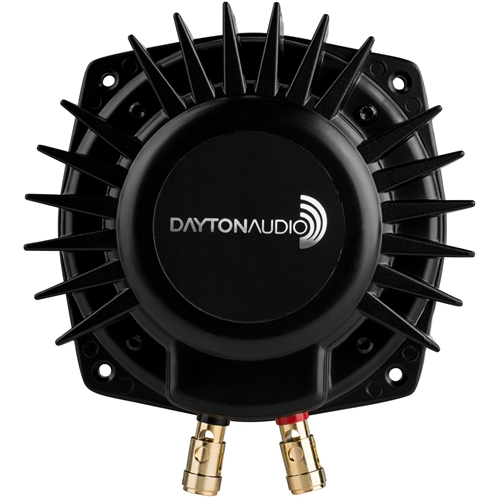
\includegraphics[width=0.4\textwidth]{images/vibrotactile_bass-shaker.jpg}
                \caption{Voice coil actuator, vibrotactile device, Dayton Audio BST-1.}
                \label{fig:VCA}
            \end{figure}

            The sensory system is a network that enables your body to receive information from the environment and its own internal state, converting stimuli into signals for the brain to process. The human sensory system doesn't just process this sensory information as a single stream; it organizes it to answer fundamental questions about the environment\cite{What_vs_Where_in_Touch}. Research in sensory neuroscience suggests a fundamental distinction in how the brain processes sensory information framed as "what" an object (disturbance) is versus "where" it is located.\par

            How do you feel the difference between rough stone, resonant wood, or soft earth? This relates directly to identifying the "what" of the surrounding environment. The "where" pathway provides spatial information, helping us to understand the location of a stimulus in relation to our body and within the environment. The location of a distant explosion felt through the floor, related to identifying "where" information.\par

            As we are exploring environmental storytelling through audio-tactile stimulation, we can extend this framework with a third component: "how". This component can include "cause and effect" relations within our sensory perception and cognition. Where "what" and "where" components answer material and spatial questions, "how" components can answer temporal questions derived from the first two components. These questions will focus on a more interactive concept of "event" rather than static stimulation characteristics.\par

            This "what, where and how" taxonomy provides a conceptual tool for environmental storytelling, thus embedding temporal relations into the environment, moving beyond simple rumbles to convey specific information about an environment's materials, spatial layouts and past/ongoing events.\par

            \begin{figure}[H]
                \centering
                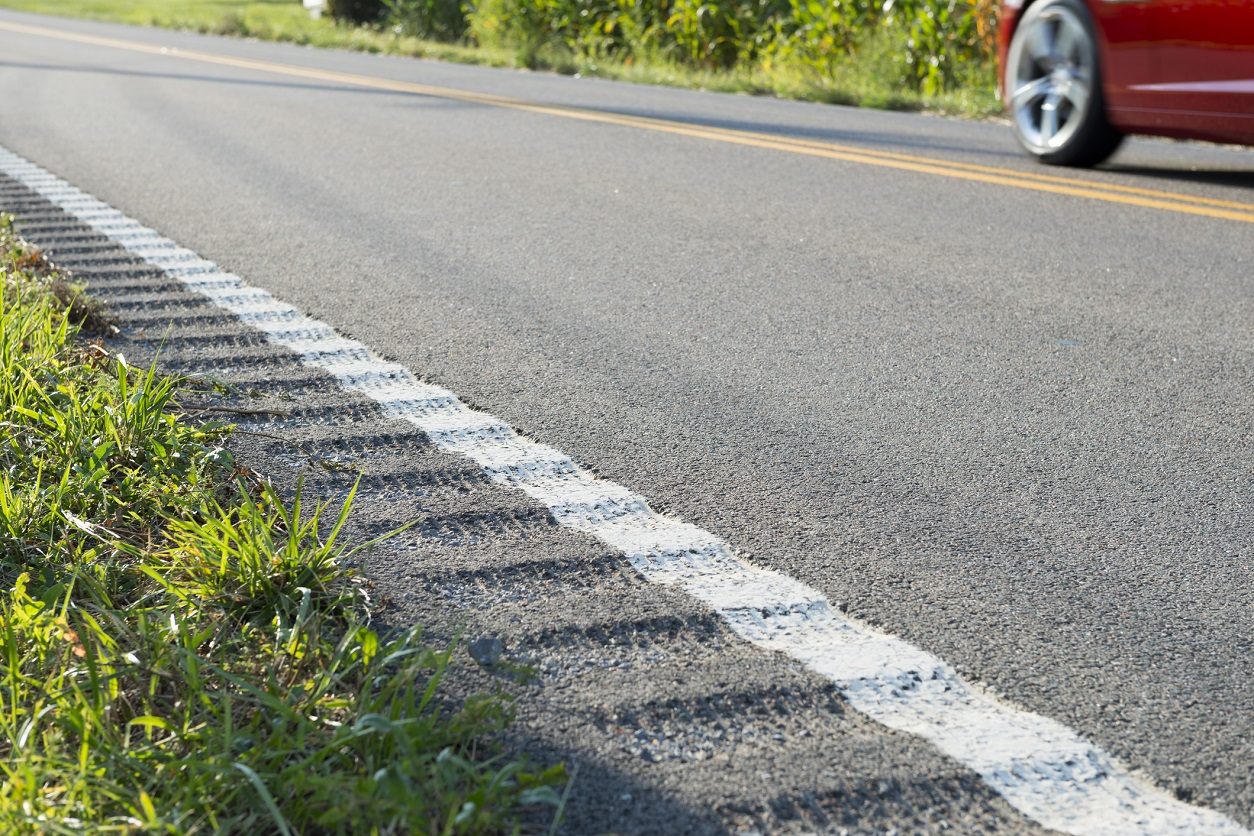
\includegraphics[width=0.8\textwidth]{images/rumble_strips.jpg}
                \caption{A visual shows road rumble strips.}
                \label{fig:RUMBLE_STRIP}
            \end{figure}

            As shown in the \ref{fig:RUMBLE_STRIP} rumble strips designed to alert drivers by creating vibrations and noise when a vehicle goes out from its intended lane or crosses the edge of the road. Stimulation from a rumble strip side of the road not just indicating physical position or a road surface information, it's an immediate warning.\par

            The sensation isn't a random patch of bad road; it's a deliberately engineered, rhythmic pattern. This pattern connects the what (the ribbed texture) and the where (the edge of the lane) to create a temporal meaning: "You are currently in the process of making a mistake." The "how" pathway interprets this sequence as a cause-and-effect event, because you are drifting, you are feeling this vibration. In a structured narrative context, this type of haptic stimulation can be utilized for environmental storytelling.\par
        \subsection{Human Tactile Perception}
            This section will cover human response to haptic stimulation, detection thresholds of vibrotactile stimulation in comparison with auditory perception.\par

            \begin{itemize}
                \item What is the detection thresholds of vibrotactile stimulation?
                \item How vibrations effect material texture feeling of an object?
                \item How whole body vibrations affect our feeling?
                \item How vibration amplitude, frequency and frequency pitch intervals effect haptic cognition?
                \item Which body parts or positions is effective in haptic stimulation most?
                \item How audio-tactile stimulation is effecting our localization capabilities?
            \end{itemize}

            These questions introduced in the context of Embracing Sphere to basically have a certain knowledge ground while crafting/designing content for Embracing Sphere. As ultimate goal is to convey an environmental storytelling through audio-tactile interface, it is crucial to explore and study haptics in detail.\par

            First answer defines tangible human limits and scales most effective playground for vibrotactile experience. Detection threshold of vibrotactile stimuli varies with frequency, transmission position and measurement conditions. Human response to vibration is multidisciplinary topic that involves many science such as biology, psychology, physics and biomechanics\cite{Human_Response_to_Vibration}.\par

            People are primarily exposed to vibration either localized or vibration that affects whole body\cite{Human_Response_to_Vibration}. We experiencing our surroundings through these 2 different vibration ways. The question, "What is the required magnitude of a vibration for it to be perceived?" has to be restructured as "What is the required magnitude of a vibration in each frequency domain for it to be perceived by hand and whole body?". This restructuring embeds more accurate investigations in human response to vibration, assembling more useful data for Embracing Sphere. In many researches\cite{Human_Response_to_Vibration}\cite{Consonance_of_Vibrotactile_Chords}\cite{Threshold_of_Stimulation_Levels}\cite{Whole-Body_Vibration_Perception_Thresholds}, vibrotactile sensitivity of hand has measured highest (lowest threshold) at mid-range frequencies (40-150Hz) and decreases (threshold increases) at very low and very high frequencies (below 20 and above 400).\par

            \begin{figure}[H]
                \centering
                \includegraphics[width=0.8\textwidth]{images/vibration_thresholds.png}
                \caption{A plotting of minimum vibration magnitude required for the hand to perceive vibration. Data collected from sources\cite{Haptic_Music}\cite{Haptic_Perception-A_Tutorial}\cite{Human_Response_to_Vibration}, plotted in matplotlib using python.}
                \label{fig:VIB_THRESHOLD}
            \end{figure}

            Whole body vibrations are important because humans are used to perceive whole vibrations in situations like being a passenger or driver in vehicles such as cars, trucks and helicopters; experiencing massive motions such as earthquake and waves in the sea\cite{Altinsoy_phd}. Whole body vibration is a vibration that affects the whole body, perceptive result of a stimuli in brain is a sum of every somatic sensors of our body\cite{Whole-Body_Vibration_Perception_Thresholds} and it may make us feel diverse feelings from nausea, sickness to refinement and rigidity\cite{Haptic_Perception-A_Tutorial}.\par 

            According to a research\cite{Perceived_Quality_with_Vibration_of_Electric_Cello} perceived quality of an instrument is slightly affected by the vibration level of an instrument and according to other studies\cite{Consonance_of_Vibrotactile_Chords}\cite{Audio-Tactile_Rendering} vibrotactile perception of musical concepts (rhythm, pitch, melody cognition) is quite similar to auditory perception.\par

            In the Audio-tactile Rendering experiment\cite{Audio-Tactile_Rendering}, tactile renderings and perceptive effects on different type of auditory concepts such as rhythm, pitch, melody, timbre and loudness explored and in the Consonance of Vibrotactile Chords experiment\cite{Consonance_of_Vibrotactile_Chords}, musical theory involved in to express musical feelings of consonance and dissonance via vibrotactile interfaces. Both experiments are highly related with my research and Embracing Sphere.

            According to study\cite{Audio-Tactile_Rendering}, tactile rhythm perception explained in a basic way of filtering the music signal and using filtered signal as an exciter for an actuator. Rhythm is described as pattern of pulses in discrete time and rhythm as a musical feature can be perceived by multiple sensory channels such as visual, auditory, and touch.\par

            Pitch perception with vibrotactile stimuli is a complex task as touch has frequency perception limitations. Simplest way is to translate pitch and loudness to vibrotactile stimuli, using speakers or VCAs which directly convert pitch to frequency and loudness to intensity of vibrations. However, frequency response of these actuators overpass skin perception thresholds we described, because of that information embedded in high-frequency bands (i.e., over 1000 Hz) might be lost.\par

            Melody builds up as a suitable combination of pitch changes over time. Therefore, most of the limitations for pitch conversion also apply to melody.\par

            Timbre allows the listener to differentiate between tones played from one or another musical instrument. Timbre relies on the frequency content called "overtones" (i.e., spectral content) of audio signals and overtones are frequencies of sound that are higher than the fundamental frequency of a vibrating object, which in a higher registry fundamental tone, an overtone series may start from higher than 600Hz. Therefore tactile translation of timbre represents a challenge.\par

            The concepts derived from music theory and composition can be utilized for creating abstract but effective audio-tactile scenes where meaning is not so direct but more intuitive.\par

            Another research\cite{Touch_the_Sound} catch my interest which experimenting an illusion that occuring during the evaluation of the multi-modal events. According to study visual, tactile and auditory information interacts and possess influence between each other. Multi-modal illusions like ventriloquism effect is an auditory illusion in which sound is misperceived from a source when it has different position at visible source. The effect is most powerful for speech sounds and it happens because of visual dominance over auditory information. It is exploited by stage ventriloquists who practice the art of speaking without moving their lips while manipulating the movements of a puppet.\cite{Touch_the_Sound}.\par
            
            \begin{figure}[H]
                \centering
                \includegraphics[width=0.6\textwidth]{images/ventriloquist.png}
                \caption{A picture of a ventriloquist Peter Kerscher. Retrieved from \url{https://commons.wikimedia.org/wiki/Category:Ventriloquism/}}
                \label{fig:VENTRILOQUIST}
            \end{figure}

            Although the multi-modal events determined by physical rules and usually has same position in physical world, it is possible to break this rules in virtual environments to have a control and optimization over object interaction in virtual environments.

            \begin{figure}[H]
                \centering
                \includegraphics[width=0.6\textwidth]{images/vibration_thresholds_02.png}
                \caption{A plotting of minimum vibration magnitude required for the localization of a vibration. Data collected from sources\cite{Haptic_Perception-A_Tutorial}, plotted in matplotlib using python.}
                \label{fig:VIB_THRESHOLD_02}
            \end{figure}            

            The localization capabilities of human with vibrotactile stimulation can be seen in the figure \ref{fig:VIB_THRESHOLD_02}.

            The sum experience of simultaneous audio and tactile stimulation is going to covered in next section but while composing an audio-tactile experience, these perceptive concepts and illusions has to be taken into account. Being able to author feelings and embed meaning utilizing this concepts is a novel way of conveying a story, in my perspective.\par
        \subsection{Haptics in Media Arts and Video Games}
            Both in media art scene and video game industry, immersion is occasionally an important subject. This section will cover several case studies in such domains that utilizing haptic feedback to translate an information, feeling or meaning.\par

            \subsubsection{Case Study: Emoti-Chair}
                The Emoti-Chair is an audio-tactile display designed to translate music, speech, and environmental noises into physical vibrations that can be felt on the body. This system is aimed at improving music accessibility for deaf and hard of hearing individuals, but it also offers a novel sensory experience for all users\cite{Emoti-Chair}.\par

                \begin{figure}[H]
                    \centering
                    \includegraphics[width=0.6\textwidth]{images/emotichair.png}
                    \caption{A visual of audio-tactile display Emoti-Chair.}
                    \label{fig:EMOTICHAIR}
                \end{figure}

                This work physically and technically one of closer works to Embracing Sphere. Both of them in core concept translating audio signals into vibrotactile stimuli via an array of voice coils actuators embedded in a chair form factor.\par

                \begin{figure}[H]
                    \centering
                    \includegraphics[width=0.6\textwidth]{images/emotichair_back.png}
                    \caption{Inside parts visual of audio-tactile display Emoti-Chair.}
                    \label{fig:EMOTICHAIR_BACK}
                \end{figure}

                Specifically Emoti-Chair using voice coil actuators that have arranged in a two-column by eight-row array can be seen in the figure \ref{fig:EMOTICHAIR_BACK}, each corresponding to a specific frequency band. This spatial mapping allows users to feel different frequency components of sound at different locations on their body.\par

                In one of the interview they have made\footnote{SmartLab TMU News, Emoti-Chair: \url{https://youtu.be/gA--cOs87p4?feature=shared}}, researchers explains the system and describing their work as its confirming the idea that music is essentially multi-modal and maybe even a-modal.\par

                \begin{figure}[H]
                    \centering
                    \includegraphics[width=0.6\textwidth]{images/emotichair_02.png}
                    \caption{A picture of audio-tactile display Emoti-Chair.}
                    \label{fig:EMOTICHAIR_02}
                \end{figure}                

                Multimodal interfaces such as Emoti-Chair incorporate multiple forms of input and output to provide a variety of devices to support human-computer interactions. In further experiments researchers introduced Emoti-Chair to professional film-makers and singers in creating and experiencing tactile music on the Emoti-Chair\cite{Composing_Vibrotactile_Music}. They reported on responses to pre and post questionnaires that collected participant views about the workshop and about vibrotactile stimulation in general.\par

                During workshops with professional film-makers, singers and artists, participants either composed vibrotactile music for the first time or experienced their voices as tactile vibrations through the Emoti-Chair. Across these diverse participants, the technology has received positive feedbacks, with strong interest in using it for future projects. Future directions include enabling artists to further explore tactile composition and developing new instruments specifically for vibrotactile music.\par
            \subsubsection{Case Study: Movement and Impact by Yvonne Weber and Sabine Haerri}
                \emph{Up to six million vehicles a year pass through the Gotthard Road Tunnel, Switzerland's most important north-south traffic artery. “Movement and Impact” gives you a completely new feeling for the Gotthard Tunnel and the cars and trucks incessantly pouring through it.\cite{Movement_and_Impact_ARS}}

                The quote above is taken from an artwork description named "Movement and Impact" co-created by Yvonne Weber, Sabine Haerri and the Ars Electronica Futurelab. I have discovered this artwork through a suggestion from my professor, Manuela Naveau and immediately I felt compelled to research further. It has exhibited in Ars Electronica Festival in 2009 and unfortunately I have no chance to experience again. I will do my best to explain the piece using the resources and visuals I have found online.\par

                \begin{figure}[H]
                    \centering
                    \includegraphics[width=0.8\textwidth]{images/movementandimpact_01.png}
                    \caption{Movement and Impact. Ars Electronica Festival in Hauptplatz Linz 2009. Foto: ARCHIPICTURE Mag. Dietmar Tollerian}
                    \label{fig:MOVNIMP}
                \end{figure}   

                In this artwork, the artists translated the heavy flow of vehicles passing through Switzerland's Gotthard Road Tunnel into a tactile experience. Sensors laid on the ground captured real-time data on traffic volume, vehicle size, weight, and direction. That data converted into gentle, rhythmic vibrations on a reclining platform\cite{Movement_and_Impact_ARS}.\par

                \begin{figure}[H]
                    \centering
                    \includegraphics[width=0.8\textwidth]{images/gotthard_tunnel.png}
                    \caption{Gotthard Road Tunnel, Switzerland.}
                    \label{fig:GOTTHARD}
                \end{figure}  

                In Movement and Impact, artists explored the translation of digital traffic data into a physical experience. Through transforming overwhelming, invisible data, they created an experience somehow intimate, tangible and even therapeutic.\par

                \begin{figure}[H]
                    \centering
                    \includegraphics[width=0.8\textwidth]{images/gotthard_map.png}
                    \caption{Openstreetview visual of Gotthard Road Tunnel, Switzerland.}
                    \label{fig:GOTTHARD_02}
                \end{figure}  

                Coincidentally I have chosen a similar practice in haptic content creation for Embracing Sphere. I recorded a bridge rumble which is emotionally close to me, Neue Eisenbahnbrücke in Linz.\par

                \begin{figure}[H]
                    \centering
                    \includegraphics[width=0.8\textwidth]{images/neue_eisenbahnbrücke.png}
                    \caption{A picture of Neue Eisenbahnbrücke, Linz.}
                    \label{fig:BRUCKELINZ}
                \end{figure}

                Since starting my master's studies at the University of Art and Design Linz, Linke Brückenstraße was my first place of accommodation. For a year and a half, I crossed this bridge nearly every morning and night. Sometimes I sat and listen waves, sometimes I put my headphones on and only felt the heavy rumble of big metal frames of this beautiful bridge.\par

                Eventually, I decided to document my experience in an auditory way. However, the experience of this bridge is far from purely auditory, so I grabbed my geophone (an electronic seismic recording device) and recorded the bridge’s rumble and the vibrations caused by passing vehicles.\par

                \begin{figure}[H]
                    \centering
                    \includegraphics[width=0.8\textwidth]{images/neue_eisenbahnbrücke_rec_01.png}
                    \caption{A picture of my recordings on Neue Eisenbahnbrücke, Linz.}
                    \label{fig:BRUCKELINZREC_01}
                \end{figure}

                \begin{figure}[H]
                    \centering
                    \includegraphics[width=1\textwidth]{images/neue_eisenbahnbrücke_rec_02.png}
                    \caption{A picture of my recordings on Neue Eisenbahnbrücke, Linz.}
                    \label{fig:BRUCKELINZREC_02}
                \end{figure}

                In conclusion, Movement and Impact was not something I knew about before making these recordings or starting to develop Embracing Sphere. However, researching this artwork has convinced me to continue along this path. I may be on the right track to express my own experience. The original files of this recording session will be used in Embracing Sphere content.\par
            \subsubsection{Case Study: Nintendo Switch and Playstation Exclusive Games}
                Both Nintendo Switch and PlayStation consoles have unique controllers. Joy-Cons for Nintendo Switch and DualSense/DualShock for PlayStation, both of them features advanced haptic feedback technologies. Many exclusive games are designed to take advantage of these features such as Astro's Playroom and 1-2 Switch.\par

                \begin{figure}[H]
                    \centering
                    \includegraphics[width=0.4\textwidth]{images/astros_playroom.png}
                    \caption{Cover visual of Playstation 5 exclusive video game Astro's Playroom.}
                    \label{fig:ASTROS}
                \end{figure}

                Astro's Playroom is an exclusive PS5 tech demo for the DualSense\footnote{Short documentary of Astro's Playroom text demo from Noclip: \url{https://youtu.be/_WpD8PvH0QA?feature=shared}}. In Astro's Playroom player can feel the texture of sand, the grittiness of ice and the tension of bow spring. Rainfall is simulated as tiny, distinct taps and pulling a bow uses adaptive triggers for realistic tension.

                \begin{figure}[H]
                    \centering
                    \includegraphics[width=0.6\textwidth]{images/dualsense.png}
                    \caption{Playstation 5 gamepad DualSense.}
                    \label{fig:DUALSENSE}
                \end{figure}

                PS5 DualSense utilizes voice coil actuators and adaptive triggers to produce complex vibration signals\cite{What_is_under_Dualsense}. Each side of the controller, there is a combination of a vibrotactile actuator, designed by Foster Electric\footnote{Commercial video of VCA from Foster Electric: \url{https://www.foster-electric.com/products/productdata/vibration_actuator_en.mp4}}.

                \begin{figure}[H]
                    \centering
                    \includegraphics[width=0.6\textwidth]{images/1-2_switch.png}
                    \caption{A picture of a game session from 1-2 Switch, an exclusive Nintendo Switch party game.}
                    \label{fig:1-2SWITCH}
                \end{figure}

                1-2 Switch\footnote{1-2 Switch Trailer Video: \url{https://youtu.be/DpHDJRGuL7w?feature=shared}} is a party game is essentially a tech demo or a showcase for HD Rumble. 1-2 Switch includes many mini games. In the “Ball Count” mini game, you “feel” virtual balls rolling inside the controller, simulating their number and movement, the "Shave" mini game, players hold the Joy-Cons as if they are a barber clipper and the Joy-Cons vibrating like the feeling of shaving facial hair. The goal is to shave a virtual beard by moving the Joy-Con in shaving motions and in the end players see who achieved the closest and cleanest shave. Except the end results the game is not relying on any visual displays, the gameplay focused only on the vibrotactile sensation from the controller.\par

                Both of the consoles and the examples that we covered is utilizing haptic capabilities of their gamepads quite intuitive. In "Chapter 1 - Introduction, Embracing Sphere and My Own Perception" section we mentioned an old technology of Playstation 2 Dualshock 2 in figure \ref{fig:Vib_Motors}, the haptic technology at that time was using weighted motors that spinning off-center to create a general rumble and it was quite low resolution and not expressive enough in comparison today's haptic technologies that uses linear resonant actuators\cite{Audio-Tactile_Rendering}. The DualSense and Joy-Cons haptic actuators are basically small speakers that can playback low frequencies clear for haptic feeling.\par
            \subsubsection{Case Study: Racing Simulations}
                Throughout my research I've explained many different inspirations that I had for the Embracing Sphere. Audio-tactile interfaces I have discovered, includes many artworks, interactive media or video games that might have been relatively linked with Embracing Sphere in concept or software/hardware side.\par

                This case study about racing simulations will cover current haptic technologies in sim-racing video games and hardwares. Additionally the section is going to be about my own experience with sim-racing and seated vibrotactile stimulation.\par

                In 2021 when I was a bachelor's student, me and my dear friend Can Memisogullari, started to play a racing game called F1 2020. At first we played through the main content that is basically raced against AI. Then after a while Can mentioned about a community that organize its own online racing league in F1 2020.\par
                
                The league organized at the Covid times and every member of the league were adults whom has a lot of free time to spend on practicing and preparing to race competitively. Looking from now it feels so absurd that we had set schedule for 10 week season, different race each week that every driver practice really hard on weekly different tracks. There was live coverage with commentary for all races and even referee committee that gets together after the race for to check the incidents happened in the race.\par

                \begin{figure}[H]
                    \centering
                    \includegraphics[width=0.8\textwidth]{images/sourleague.png}
                    \caption{A visual from F1 2021 game, online sim-racing league I attended in 2021.}
                    \label{fig:SOURLEAGUE}
                \end{figure}

                First season, me and Can raced with a generic gamepads and there was a distinction between players who use gamepad and players who use force feedback (FFB) wheels. FFB wheel users were basically faster and more consistent in vehicle control. Of course there is more than one parameter different between gamepad and FFB wheel but there was the consensus in the community that the pace different is coming from feeling of the vehicle.\par

                \begin{figure}[H]
                    \centering
                    \includegraphics[width=0.6\textwidth]{images/ffb_image.png}
                    \caption{A visualization, inside of a belt driven force feedback wheel system.}
                    \label{fig:FFB}
                \end{figure}

                FFB is a technology used in racing simulation hardware, especially in steering wheels, to provide physical sensations that mimic real-world driving. FFB wheels use motors and sensors to generate resistance, vibrations, and subtle movements that reflect what is happening with the car in the game. This feedback allows the player to feel important information, such as:\par

                \begin{itemize}
                    \item The grip level of tires.
                    \item Road surface texture (bumps, kerbs, gravel traps)
                    \item Weight transfer of the car while cornering, braking and accelerating.
                \end{itemize}
                When racing with a gamepad, the only feedback coming from visual and sometimes subtle vibration cues. This makes it harder to judge the car's behavior, especially at the limit. With an FFB wheel, the physical sensations are much richer and more detailed. This difference is why FFB wheel users tend to be faster and more consistent in sim-racing league.

                With that information I decided to buy myself a FFB wheel. The wheel I bought was belt-driven Thrustmaster T300 RS GT as seen in the figure. \ref{fig:SIMRIG}. 

                \begin{figure}[H]
                    \centering
                    \includegraphics[width=0.6\textwidth]{images/simrig.png}
                    \caption{A picture of my simulation rig, Thrustmaster T300 RS GT.}
                    \label{fig:SIMRIG}
                \end{figure}

                My experience after I adapted my driving style and muscle memory to a wheel that I've started to see improvements in my peak pace and overall consistency around track. I believe it is mostly because of constant vehicle state information stream to my nervous system with FFB. I could feel the loosing grip on back tires when I made a mistake out of corner. The more interesting part I started to make real life reactions to vehicle behavior such as counter steering and brake pressure managements\footnote{A short clip of my driving and counter steering to loosing back of my car in the online sim-racing league: \url{https://www.twitch.tv/mehmetcolak/clip/KnottySmoothJuiceCclamChamp-5y_nOCkwwXRh4bjq}}.

                Sim-racing softwares (racing video games) are developed realism taken into account and sim-racing games are benchmark for immersive experiences in the gaming industry, especially through their advanced use of haptic feedback. Video games such as iRacing and BeamNG.drive are renowned for their realistic simulation of vehicle dynamics, which is later integrated to haptic hardwares such as FFB wheels and bass shakers.\par

                These simulation games are designed to take full advantage of haptic hardware. For example iRacing provides highly detailed telemetry data that is used by force feedback systems to replicate real-world car behavior. Third party softwares can receive this telemetry data, evaluate and output a haptic feedback signal stream. This integration make the player feel every bump, skid and collision.\par

                \begin{figure}[H]
                    \centering
                    \includegraphics[width=0.8\textwidth]{images/vrs_telemetry.png}
                    \caption{A visual of user interface of a third party telemetry software for iRacing.}
                    \label{fig:VRS}
                \end{figure}

                Since 2021 I followed the technological developments in sim-racing softwares and hardwares. As my experience directs I believed that it is really immersive and most of the reason of immersion was coming from haptic feedback that has evaluated through simulation telemetry data. Because of that in Embracing Sphere, I chose to utilize a similar setup to create virtual environment for navigating and exploring.\par
            \subsubsection{Case Study: Feelies in Brave New World by Aldous Huxley}    
                Brave New World, is a dystopian novel by English author Aldous Huxley. He has written Brave New World in 1931 and published in 1932\cite{Brave_New_World}. The story begins in a distant future London, where people are engineered and conditioned from birth into fixed classes: Alpha, Beta, Gamma, Delta, and Epsilon. Embryos are chemically altered to suit their future roles. Higher classes are genetically enhanced, while lower-class citizens are deliberately impaired. Each class is trained/conditioned to accept its status, wears distinct clothing and fulfills specific societal functions such as leadership or manual labor.\par

                \begin{figure}[H]
                    \centering
                    \includegraphics[width=0.8\textwidth]{images/bravenewworld.png}
                    \caption{Cover visual of Brave New World by Aldous Huxley. Publication from Harper Perennial.}
                    \label{fig:BRAVENEWWORLD}
                \end{figure}

                In Brave New World, a distinctive imaginary multi-sensory entertainment medium called the "feelies" is introduced. This sensory apparatus serves as a cinema-like experience but unlike conventional cinema, it incorporates not only sight and sound but also smell and touch. The feelies are depicted as one of the society's control mechanisms, alongside drugs like "soma" and sleep-learning techniques "hypnopaedia."\cite{Pleasure_of_Modernism}. The masses kept under control and satisfied using feelies as an amusement tool within the theme of sensory colonization\cite{Feelies}.\par

                According to Grossi\cite{Feelies}, the fantasy of total sensory cinema is deeply tied to the configuration of a mass society and the programming of human psyche. The pejorative descriptions of these technologies aside, the idea of an enhanced multi-sensory medium and imagining this during the golden age of real-world cinema fascinated me. Even today, the development of immersive media continues to involve the direct "colonization" of human sensory fields such as virtual reality and augmented reality technology advancements.\par

                Eventually, Embracing Sphere can be seen as re-evaluation or re-imagination of many of these examples discussed in the section "Haptics in Media Arts and Video Games". As the artist behind this project, I have tried my best to be honest and true to my own creation. Practicing artistic/scientific research about my work was the main control system of my artistic outputs, provided me many references in my domain and my pursuit. With the inspirations covered in detail this section, the next chapter "Personal Project, System Design and Methodology" will detail concept and design features of Embracing Sphere.\par